\documentclass{article}

\usepackage[margin=1in,left=1.0in,includefoot]{geometry}
\usepackage{graphicx}
\graphicspath{ {./images/} }

\usepackage{fancyhdr}
\pagestyle{fancy}
\fancyhead{}
\fancyfoot{}
\fancyfoot[R]{ \thepage\ }
\renewcommand{\headrulewidth}{0pt}
\renewcommand{\footrulewidth}{1pt}

\begin{document}

\begin{titlepage}
	\begin{center}
	\huge{\bfseries COSC2149 Research Methods} \\
	[0.5cm]
	\Large{\bfseries Assignment 3: Final thesis proposal} \\
	[0.5cm]
	\end{center}
	\begin{flushleft}
	\[
	\begin{array}{ll}
	\normalsize
	\textbf{Student:} & \textup{Tyler Saxton (s3768946@student.rmit.edu.au)}\\
	\textbf{Primary Supervisor:} & \textup{Dhirendra Singh}\\
	\textbf{Program:} & \textup{Master of Data Science} \\
	\textbf{Title:} & \textup{Auditing safety of on-road cycling infrastructure using Google Street View and deep learning} \\
	\end{array}
	\]
	\end{flushleft}
\end{titlepage}

\section{Introduction}

The benefits of ``active transport'', such as walking and cycling, have been well documented in previous studies.  Participants' health may improve due to their increased physical activity.  There are environmental benefits due to reduced emissions and pollution.  And there are economic benefits, including a reduced burden on the health system, and reduced transportation costs for participants \cite{LEE2012219} \cite{RABL2012121}.
\\

Federal and State government policy makers in Australia therefore wish to encourage cycling \cite{federal_policy_2019} \cite{state_policy_2020}.  However, the share of cycling for trips to work in Melbourne is only 1.5\% \cite{melbactive}.  For many commuters, a perceived lack of safety of cycling is a major barrier to adoption.  Other significant factors are the availability of shared bicycle schemes, storage facilities, and the risk of theft \cite{WILSON2018234}. Cycling infrastructure has a significant impact on real and perceived cyclist safety, and this research project will focus on that issue.  Important safety factors include the presence and width of a bicycle lane, the presence of on-street parking, downhill and uphill grades, and the quality of the road surface \cite{BIKESAFETY} \cite{Teschke2012}.  A comprehensive dataset of cycling infrastructure would help policy makers identify and prioritize areas in need of improvement to safety.
\\

The aim of this research project is to investigate whether cycling infrastructure can be measured and recorded by applying a machine learning classifier to street scene images sourced from Google Street View.  The focus will be on detecting the presence and width of a bicycle lane on a road, through semantic image segmentation.
\\

If we are able to reliably detect the cycling infrastructure via machine learning and street scene images, then we will investigate whether we can create a process or workflow to ``tudit'' cycling infrastructure on all roads in a local area, to build a dataset. \\

Additional characteristics of cycling infrastructure that are important for cyclist safety are presented below, in the literature review.  It may be possible to detect or quantify some of these with machine learning too, in extended or future work. \\

Google Street View has been chosen as a source of street scene image data due to its wide geographical coverage, and the accessibility of the data via an API.  However, the images for any given location might be several years out of date.  This will be taken into consideration when evaluating any machine model against a source of ``ground truth''.  If the research is successful, then a local government responsible for building and maintaining road infrastructure could gather their own up-to-date imagery, at regular intervals.

\section{Research Questions}
\begin{enumerate}
\item{Can machine learning be used to identify bicycle lanes in street view imagery sourced from Google Street View?}
\item{Can the width of the detected bicycle lanes be estimated based on the width of the pixels involved, and photogrammetry?}
\item{Can the model then be used to detect and measure bicycle lanes across all streets in a local area with Google Street View coverage?}	
\end{enumerate}

\cleardoublepage

\section{Literature Review}
\subsection{Motivation}

Prior research has clearly shown health, economic, and environmental benefits from active transport:
\begin{itemize}
\item{Lee et al., 2012 \cite{LEE2012219} analysed World Health Organization survey data from 2008, and showed that physical inactivity significantly increased the relative risk of coronary heart disease, type 2 diabetes, breast cancer, colon cancer, and all-cause mortality, across dozens of countries.}
\item{Rabl \& de Nazelle, 2012 \cite{RABL2012121} demonstrated that active transport by walking or cycling improves those relative risks for participants.  Moderate to vigorous cycling activity for 5 hours a week reduced the all-cause mortality relative risk by more than 30\%.  They estimated an economic gain from improved participant health and reduced pollution, offset slightly by the cost of cycling accidents.}
\end{itemize}

In Australia, Federal and State governments are committed to the principle of supporting active transport through the provision of cycling infrastructure, declaring their commitment through public statements on their official websites \cite{federal_policy_2019} \cite{state_policy_2020}.  Many other governments around the world have adopted similar policies.
\\

Taylor \& Thompson, 2019 \cite{melbactive} surveyed the use of active transport in Melbourne, to establish a baseline of current commuter behaviour.  They found that cycling only accounted for 1.5\% of trips to work in the area.  It could therefore be argued that there is room for improvement.
\\

Schepers et al., 2015 \cite{SCHEPERS2015460} produced a summary of literature related to cycling infrastructure and how it can encourage active transport, resulting in the aforementioned benefits.  The paper found that providing cycling infrastructure that is perceived as being safer does encourage participation.  Other papers such as Wilson et al., 2018 \cite{WILSON2018234} agreed.
\\

Other researchers have examined which factors affect the perceived and actual safety of cycling routes:
\begin{itemize}
\item{Klobucar \& Fricker, 2007 \cite{BIKESAFETY} surveyed a group of cyclists in Indiana, asking them to ride a particular route and rate the safety of each road segment along the route, then asking them to review video footage of other routes and rate the safety of those routes, too.  A regression model was created to predict the cyclists' likely safety ratings for other routes.  The creation of the model led to a list of road segment characteristics that were apparently most influential in the Indiana setting.}
\item{Tescheke et al., 2012 \cite{Teschke2012} surveyed patients who attended hospital emergency rooms in Toronto and Vancouver due to their involvement in a cycling accident.  Details of the circumstances of each accident were gathered, along with the outcomes.  The data was analysed to determine which factors increased (or decreased) the relative odds of a cyclist being involved in an accident.}
\item{Malik et al., 2021 \cite{Malik2021} modelled cyclist safety in Tyne and Wear County in north-east England, a more rural setting.}
\end{itemize}
The factors that contribute to cyclist safety vary by locality.  For example, cyclists in one city might be concerned by the hazard of tram tracks, whereas this might not be a relevant concern in another city, or a less built-up area.  The common themes were:
\begin{itemize}
\item{Presence and type of bicycle lane (dedicated, paved shoulder, none)}
\item{Width of bicycle lane}
\item{Presence of on-street parking}
\item{Downhill or uphill grades}
\item{Volume, speed, and vehicle type profile of motor vehicle traffic}
\item{Quality of road surface (including drainage, tram tracks, etc.)}
\item{Lighting}
\item{Construction Work}
\end{itemize}
Most of these factors can be influenced by infrastructure and road design.  Therefore, it would be valuable to quantify as many of these factors as possible in a dataset, to assist policy makers in deciding what changes ought to be made, and where, to provide a safer network of cycling infrastructure.
\\

\subsection{Applications of Machine Learning}

Semantic image segmentation of street scene images is an important and active area of computer science research.  ``Deep Learning'' models that can understand sequences of images in real time are essential for self-driving vehicles or similar driver-assistance systems, so many papers have focussed on that area.
\\

Papers by Cordts et al., 2016 \cite{Cordts_2016_CVPR} and Zhou et al., 2019 \cite{ade20k} announced the publication of the ``Cityscapes'' and ``ade20k'' image datasets, respectively.  These datasets each contain many street scene images, with objects of interest labelled in a format suitable for training deep learning models to understand similar on-road scenarios.  Many papers have used these datasets in order to train new machine learning models.  Unfortunately, neither of the datasets has cycling infrastructure labelled.  The ``CityScapes'' dataset has labelled bicycle lanes under the ``sidewalks'' category.  This is useful to train a car not to drive there, but a cyclist might not be legally allowed to ride on a sidewalk designed for pedestrian traffic.
\\

Chen et al., 2018 \cite{DEEPLAB} is one example of a heavily-cited paper where ``CityScapes'' data has been used to train a ``real time'' model to understand on-road video footage.
\\

Other papers provide background on the ``Deep Learning'' tools that are being applied to street scene understanding, and the theory behind them:
\begin{itemize}
\item{Ren et al., 2015 \cite{REN2016} R-CNN}
\item{He at al, 2016 \cite{He_2016_CVPR} ResNet}	
\item{Abadi et al., 2016 \cite{TENSORFLOW2016A} \cite{TENSORFLOW2016B} TensorFlow}
\item{Paszke et al., 2019 \cite{passing_space} PyTorch}
\end{itemize}

In another branch of research, deep learning tools have been used to manage roadside infrastructure and assets:
\begin{itemize}
\item{Campbell et al., 2019 \cite{CAMPBELL2019101350}	 used an ``SSD MobileNet'' model to detect ``Stop'' and ``Give Way'' signs on the side of the road in Google Street View images, to help build a database of road sign assets.  An application called ``RectLabel'' was used to label 500 sample images for each type of sign.  Photogrammetry was used to estimate a location for each detected sign, based on the Google Street View camera's position and optical characteristics and the bounding box of the detected sign.}
\item{Zhang et al., 2018 \cite{s18082484} performed a similar exercise, detecting road-side utility poles using a ``ResNet'' model.}
\end{itemize}

The use of satellite imagery and aerial photographs were also considered.  Li et al., 2016 \cite{ROADNETWORK} showed that a road network could be extracted from satellite imagery using a convolutional neural network (CNN), and this is particularly useful in rural areas where maps are not already available.  However the resolution of available satellite image data would not be sufficient to identify a bicycle lane on a road.  Satellite imagery may have a role to play in detecting off-street bicycle tracks in ``green'' parkland area, but it was decided to exclude that from the scope of this research.
\\

Aerial photography may be useful, where it is available with sufficient detail.  However it would require a different data source for every jurisdiction.  Ning et al., 2021 \cite{NING2021} had success extracting sidewalks from local aerial photography using a ``YOLACT'' model.  Areas of uncertainty caused by tree cover were filled in using Google Street View images.  The model appeared to rely on a concrete sidewalk having a very different colour to the adjacent bitumen road.  The approach might not be able to distinguish bitumen bicycle lanes.  The road markings were not visible.
\\

Rita, 2020 \cite{rita_2020} used the ``MS Coco'' and ``CityScapes'' datasets to train ``YOLOv5'' and ``PSPNet101'' models to identify various classes of object (Bicycle, Car, Truck, Fire Hydrant, etc.) in Google Street View images of London.  A matrix of correlations between objects was calculated.  This was used to infer the circumstances where cyclists might feel the most safe.  For example, there was a high correlation between ``Person'' and ``Bicycle'' which ``suggests pedestrians and cyclists feel safe occupying the same space''.
\\

Chen et al., 2018 \cite{7784064} is one of many papers from the autonomous vehicle research domain that uses a Canny Edge Detector and Hough Transform to detect lane markings.   Mamidala et al., 2019 \cite{8929655} used a CNN model to detect the outer boundary of a road.


\subsection{Available Cycling Infrastructure Datasets and Standards}

\begin{itemize}
\item{In Victoria, the State Government started publishing an official ``Principal Bicycle Network'' dataset in 2020 \cite{PrincipalBicycleNetwork}.  It includes current and planned bicycle routes.  There is a field to record the width of a bicycle lane to the nearest metre, but it is not always populated.  Many entries have been marked as last being ``validated'' in 2014, or not at all.  The dataset only covers formal bicycle lanes, so it excludes roads where the cyclist may ride on a less formal paved shoulder, separated from the lanes used by vehicles.}
\item{``OpenStreetMap'' \cite{OPENSTREETMAP} is a source of crowd-sourced map data, and it supports ``cycleway'' tags where contributors can mark not just where a bicycle lane is, but its attributes, such as whether it is shared with public transport, whether there is a specially marked area for cyclists to stop at intersections, and how wide the bicycle lane is.  Given that the data is crowd-sourced, the quality and availability of the data may vary by location.}
\item{``Google Maps'' provides a ``bicycle layer''.  This includes off-street bicycle paths and on-street bicycle lanes.  It only gives a ``yes'' or ``no'' opinion about whether a route is especially suited to bicycles, with no further information provided.  But that may be of assistance in scouting locations to use in a training dataset of Google Street View images.}
\item{Other services such as ``Strava'' and ``Trailforks.com'' hold data that cyclists have recorded about their rides.  These may be useful to assess the popularity of routes, and perhaps infer where upgrades would be welcomed, or where there might be an existing route that should be checked and added to a dataset.}
\item{The Victorian Government publishes an open database of address information \cite{vicmap}, which is useful for iterating over every street in a local area.}
\item{The Supplement to Australian Standard AS1749.9 \cite{as1742} provides information on the standards by which bicycle lanes are constructed and marked in Australia.}
\end{itemize}

\cleardoublepage


\section{Methodology and Project Plan}

Work on this research project will be conducted throughout the 2021 academic year.  During Semester 1, we worked towards this final research proposal, where the research questions were determined, the literature review was conducted, and a plan set in place for the rest of the project.  Implementation, evaluation, and thesis report writing will primarily happen during Semester 2.  However the semester break can also be used to accelerate the timeline and thereby make it easier to respond to issues.  See Figure 1 for an overview of the planned Project Timeline:
\\
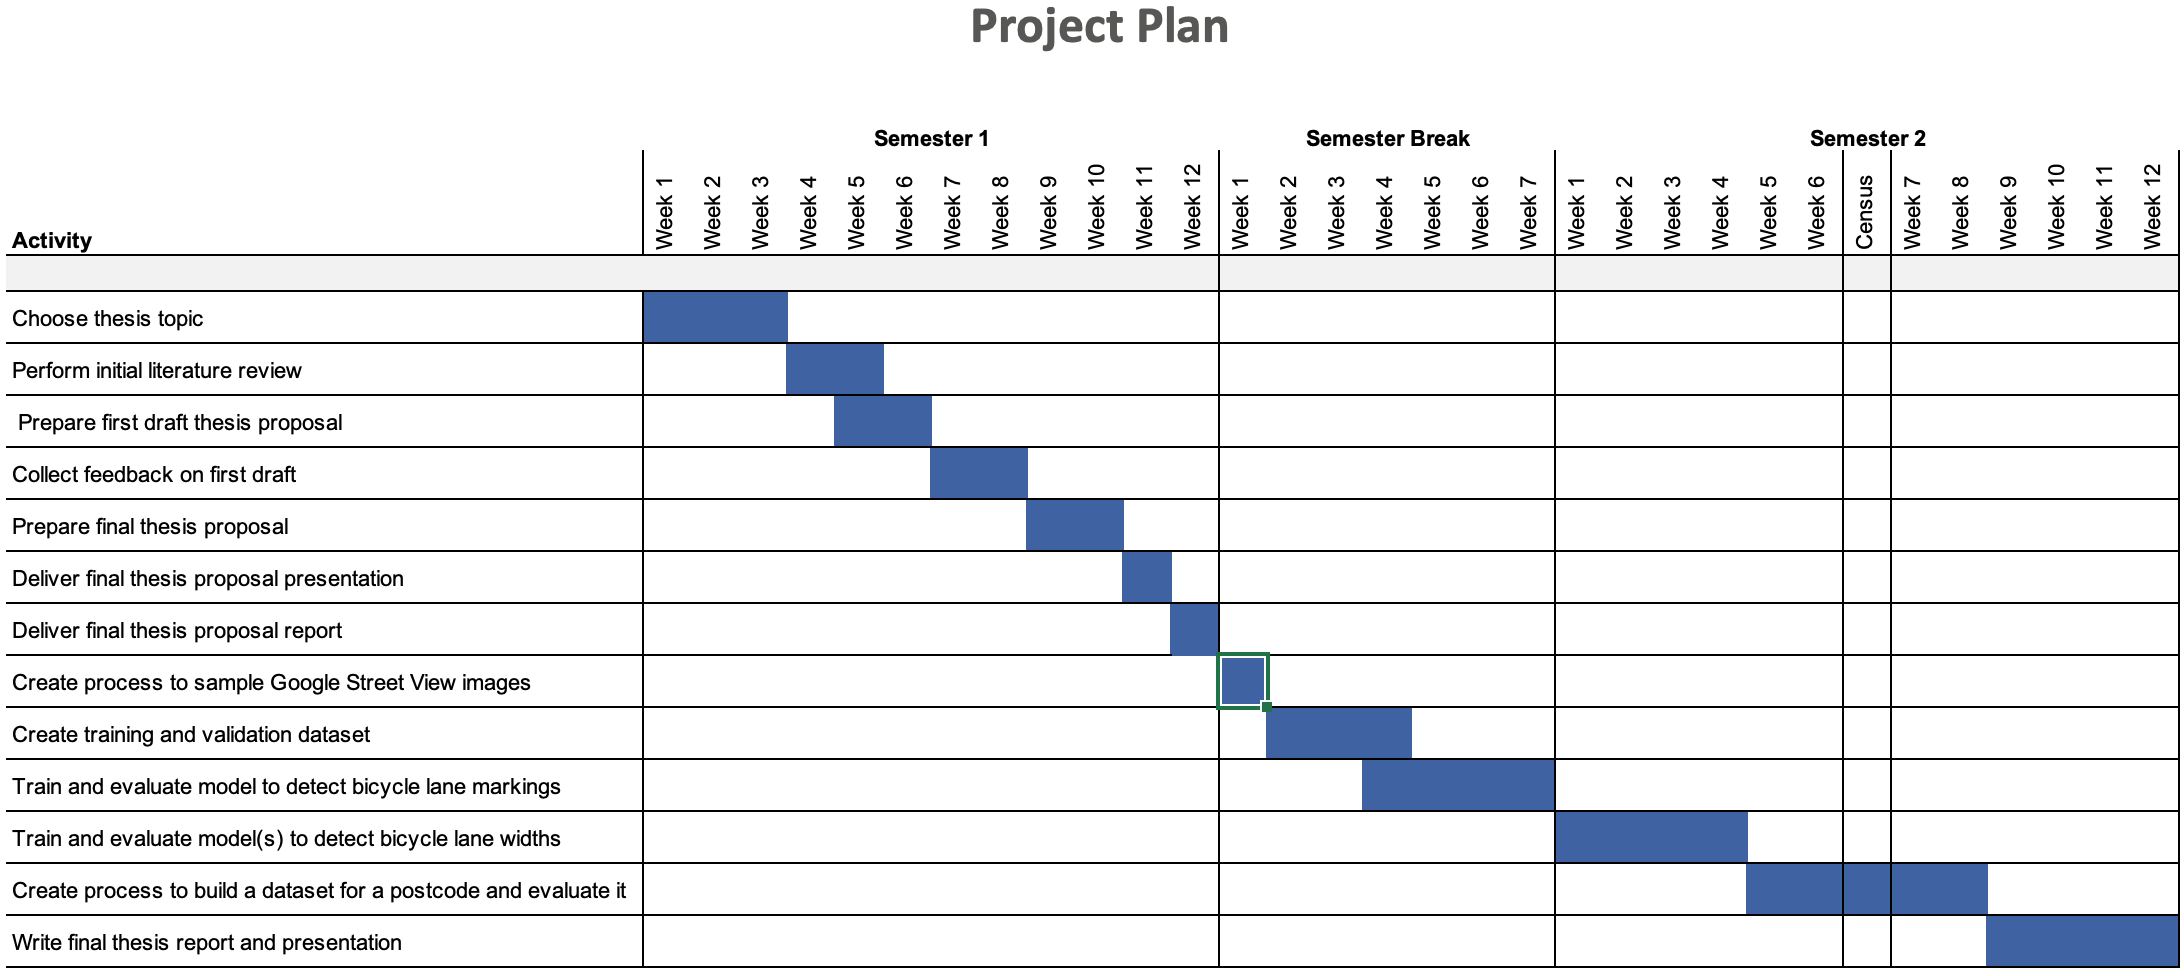
\includegraphics[width=\textwidth]{ProjectPlan005.png}

\textit{Figure 1: Project Timeline}
\\

The intent is to complete the research project in Semester 2, 2021 in COSC2179 Minor Thesis/Project.  However, as a part-time student, there is an option transfer to COSC2389 Minor Thesis/Project Part A and complete the project in Semester 1, 2022, if insufficient progress is made by the Census Date between Week 6 and Week 7.  No other subjects will be undertaken in parallel, as delivery of the Minor Thesis is the only remaining requirement to complete the Master of Data Science degree.\\

The first major milestone will be to create a training dataset, and then train a model to recognise the road markings that appear on an official bicycle lane.  See Section 6 for a detailed breakdown of the tasks to achieve this.  The project plan calls for this to be completed during the break between Semester 1 and Semester 2, if possible. \\

Campbell et al., 2019 \cite{CAMPBELL2019101350} constructed training datasets with 500 images of each sign they wished to detect.  It is anticipated that we will need to construct a training dataset of a similar size, to detect bicycle lane markings.  We will use knowledge of the Australian standards for bicycle lane construction \cite{as1742} and address data from the ``Principal Bicycle Network'' dataset \cite{PrincipalBicycleNetwork} to gather a list of streets where bicycle lane markings are likely to appear.  Bicycle lane markings are required 15 metres from each road intersection, with additional markings every 200 metres or less.  Knowing where they are supposed to be will increase our chances of finding suitable images for the training dataset quickly.  The OpenStreetMap API can be used to gather a list of intersections per street.  Once we have a randomly selected list of intersections to sample, we will use the the Google Street View API to download images at the intersection and up to 200 metres down the road.  We can then use a labelling tool to go through the images and apply labels. \\

We will train a deep learning model to detect the bicycle lane markings \textit{as we are constructing the test dataset}, evaluating after we have labelled 100, 250, 500, etc. images to determine when we appear to have sufficient training data to achieve satisfactory performance.  These initial evaluations will be performed by ``holding out'' a proportion of the training data, and  seeing whether the models correctly predict the number of bicycle lane markings that appear (compared to the labels) and then whether they appear in the same area of the image.  \\

Once we are getting satisfactory results in detecting the bicycle lane markings, we will need to apply other methods to estimate the width of the bicycle lane.  OpenCV implementations of a Canny Edge Detector + Hough Transform should hopefully allow us to detect the lane markings, similar to work done by Chen et al., 2018 \cite{7784064} as an example.  Bicycle lanes typically border on the outer-most part of a road surface.  If the aforementioned approach is not sufficient to identify the outer edge of the bike lane -- due to variations in the surface next to the roads -- then it might be necessary to replicate the techniques of Mamidala et al., 2019 \cite{8929655}, who used a CNN model to detect the outer boundary of a roadway.  The standard training datasets CityScapes \cite{Cordts_2016_CVPR} or ade20k \cite{ade20k} might help us train models to solve this problem. \\

If we know where a bicycle lane marking is, and we can find its bounding lane markings, then we should be able to use photogrammetry to determine its width.  Campbell et al., 2019 \cite{CAMPBELL2019101350} did something similar to give a precise location to ``Stop'' and ``Give Way'' signs found in the image.  For each image, we know where the camera was, which way it was pointed, and we also have information about its optics.  This should be enough to provide an estimate of the lane width. \\

Four weeks have then been allocated to write the final thesis report, and prepare a final presentation.


\section{Evaluation}

This research project will follow a ``build'' methodology:  The aim is to build an artefact -- a model to detect and measure the width of bicycle lanes in street scene images -- to demonstrate that it is possible.
\\

During the literature review, no prior research to deliver an equivalent system was found.  This project will review previous research to identify and locate objects in street scene images, and then apply similar techniques to a different problem.
\\

In Victoria, Australia, there is an existing, official ``Principal Bicycle Network'' dataset.  This will be used as a source of ``ground truth'' to help train the model.  The model could then be applied to other locations where data on bicycle lanes is more scarce.
\\

A training and validation dataset will be constructed, to identify and label bicycle lanes in one local area of Melbourne.  The dataset must include scenes with and without a bicycle lane.  The dataset will be split into training and validation subsets to measure the ability of the model to identify which images contain a bicycle lane, compared to what was manually labelled.  A sample of the positive matches will be reviewed, to ensure that the model is accurately identifying the pixels of each bicycle lane within the image, or a bounding box that might be used to measure the width.
\\

Once a model has been validated against the labelled dataset, it can be applied to a different local area within Melbourne.  Streets will be sampled by iterating through a database of property addresses within a postcode.  The results will be compared to the ``ground truth'' of the ``Principal Bicycle Network'' dataset.  A sample of differences will be manually reviewed and investigated.  Some differences may arise from timing issues:  When was the Google Street View image last updated, and when was the ``Principal Bicycle Network'' dataset last updated.  According to Google's published schedule, Google Street View images for Melbourne will be updated throughout 2021 \cite{googleschedule}.  Other differences may arise from limitations in what is visible from the Google Street View camera.  For example, there may be a bike lane on a ``service road'' where the marking are not visible from the lane that the camera was driven down.  A workflow will be created to quickly  sample and review as many differences as possible, and note the cause of each difference so that these can be measured separately.
\\

Estimations of the width of a detected bicycle lane will be compared to the Principal Bicycle Network for an official measurement to the nearest metre (when recorded).  It may also be possible to compare to ``cycleway'' tags in OpenStreetMap.  Otherwise, a small training and validation dataset will be created where widths have been measured in person for the research project, and are therefore known.  The ``Principal Bicycle Network'' data can help identify candidate streets with different width bicycle lanes, to include in the dataset.

\section{Preliminary Work / Results}

This research project is being undertaken on a part-time basis.  Work to-date has focussed primarily on preparing a final research proposal, with most implementation work expected to commence in the break between Semester 1 and Semester 2. \\

The ``Principal Bicycle Network'' dataset \cite{PrincipalBicycleNetwork} and a full dataset of Victorian addresses \cite{vicmap} have been downloaded, and successfully read into Python from their Excel and DBF file formats. \\

The next steps involve interfacing to datasets and services to create a workflow for building a dataset to train a model to detect bicycle lane markings.  We would like to create a process to help us download Google Street View images for locations where we are likely to find the markings quickly, and store them in an appropriate structure, ready to be labelled. \\

According to the Australian standards, we expect to find the markings 15 metres before and after every intersection, with additional markings spaced no more than 200 metres apart \cite{as1742}.  The ``Principal Bike Network'' dataset can tell us which roads we are likely to find the markings on.  The OpenStreetMap API provides an easy method to get a list of intersecting roads.  We can then use the Google Street View API to download a set of images for each of these intersections, including a sequence of images up to 200m further up the road, to capture some mid-segment markings. \\

Notes have been taken about areas where unusual bicycle lanes can be found, e.g.:
\begin{itemize}
\item Bicycle lanes in service roads (e.g. Royal Parade, Parkville) where we may need to use a side-facing image to detect the symbol
\item Bicycle lanes that transition between bitumen shared with the roadway and concrete that looks like a footpath (e.g. Sladen Street, Cranbourne)
\item Bicycle lanes where the marking is partially occluded and/or there is no solid white line marking a boundary (e.g. Mountain Avenue, Mount Eliza)
\end{itemize}

Some such addresses may be manually added to the sample address lists for the training data, to ensure that these scenarios are covered. \\

Campbell et al., 2019 \cite{CAMPBELL2019101350} found that they needed to create training datasets with 500 images of each street sign type they wanted to detect.  It is anticipated that the training dataset will need to be a similar size. \\

Once we have images for a training dataset, we can then work our way through labelling the images with a tool such as ``RectLabel'', which has been purchased from the Mac OS App Store, and briefly tested. \\

We will then start training a model to detect the bicycle lane markings.  The choice of initial model will be influenced by what appears to have been successful in related work that was uncovered in the literature review, and what has already been used successfully in other recent coursework. \\


\section{Expected Outcomes}

The expected outcomes of this project are:
\begin{itemize}
\item{A dataset of Google Street View images will be created from a local area in Melbourne, Australia, for the purposes of training and validating a model to detect and measure bicycle lanes.}
\end{itemize}

This will lay the groundwork for addressing all three research questions.
\\

It is similar in concept to the ``CityScape'' \cite{Cordts_2016_CVPR} and ``ade20k'' \cite{ade20k} datasets, except on a much smaller scale, due to resource constraints.  The Google Maps ``bicycle'' layer and the ``Principal Bicycle Network'' dataset will be used as a guide to which streets to sample for images containing bicycle lanes.  For each street that is sampled, images may be sampled from multiple points on the street, if the chosen Deep Learning tool is likely to be able to take advantage of that to reduce uncertainty.  The number of required images will be discussed with the research project supervisor.  As a rough guide, in Campbell et al., 2019 \cite{CAMPBELL2019101350} it was sufficient to sample 500 images of each type of road sign.  Sample images will be labelled with the ``RectLabel'' tool (available on Apple's Mac App Store).
\\

There is a risk that this task may take a very long time to complete, depending on how many images are required, and how long it takes to label each one.  To mitigate the risk, work on this task will start early, in the break between semesters.

\begin{itemize}
\item{At least one model (e.g. DeepLabv3, YOLOv5) that has been trained to detect bicycle lane markings, and evaluated against independent validation images to measure performance.}
\end{itemize}

This item will address the first research question.
\\

When the dataset is split into training and validation subsets, they will be separated by sample street, so that the multiple samples per street remain together.  If time permits, multiple Deep Learning tools will be trialed, however the first one will be chosen based on what appears most likely to succeed within the project timeline, based on recent literature.

\begin{itemize}
\item{An extension to the above model that will estimate the width of a detected bicycle lane, based on the width of the region identified in the image, documented characteristics of the Google Street View camera, and photogrammetry.}
\end{itemize}

This item will address the second research question.
\\

\begin{itemize}
\item{A process or workflow to apply the best-performed model to a new local area within Melbourne, Australia, and build a dataset of bicycle lanes and their widths on each road segment.}
\end{itemize}

This item will address the third research question.
\\

The model(s) will be carefully evaluated to determine whether it is producing useful and reliable results.  If it is not possible to achieve that, the findings will be documented along with an explanation of the challenges, and the focus of the research might then shift to another cycling safety factor.  Implementation work will commence during the break between semesters, to mitigate this risk as much as possible.
\\


\cleardoublepage
\bibliographystyle{IEEEtran}
\bibliography{references.bib}
	
\end{document}